\documentclass[12pt, titlepage]{article}

\usepackage{fullpage}
\usepackage[round]{natbib}
\usepackage{multirow}
\usepackage{booktabs}
\usepackage{tabularx}
\usepackage{graphicx}
\usepackage{float}
\usepackage{hyperref}
\hypersetup{
    colorlinks,
    citecolor=blue,
    filecolor=black,
    linkcolor=red,
    urlcolor=blue
}

%% Comments

\usepackage{color}

\newif\ifcomments\commentstrue %displays comments
%\newif\ifcomments\commentsfalse %so that comments do not display

\ifcomments
\newcommand{\authornote}[3]{\textcolor{#1}{[#3 ---#2]}}
\newcommand{\todo}[1]{\textcolor{red}{[TODO: #1]}}
\else
\newcommand{\authornote}[3]{}
\newcommand{\todo}[1]{}
\fi

\newcommand{\wss}[1]{\authornote{blue}{SS}{#1}} 
\newcommand{\plt}[1]{\authornote{magenta}{TPLT}{#1}} %For explanation of the template
\newcommand{\an}[1]{\authornote{cyan}{Author}{#1}}

%% Common Parts

\newcommand{\progname}{ProgName} % PUT YOUR PROGRAM NAME HERE
\newcommand{\authname}{Team \#, Team Name
\\ Student 1 name
\\ Student 2 name
\\ Student 3 name
\\ Student 4 name} % AUTHOR NAMES                  

\usepackage{hyperref}
    \hypersetup{colorlinks=true, linkcolor=blue, citecolor=blue, filecolor=blue,
                urlcolor=blue, unicode=false}
    \urlstyle{same}
                                


\newcounter{acnum}
\newcommand{\actheacnum}{AC\theacnum}
\newcommand{\acref}[1]{AC\ref{#1}}

\newcounter{ucnum}
\newcommand{\uctheucnum}{UC\theucnum}
\newcommand{\uref}[1]{UC\ref{#1}}

\newcounter{mnum}
\newcommand{\mthemnum}{M\themnum}
\newcommand{\mref}[1]{M\ref{#1}}


\newcounter{reqnum} %Requirement Number
\newcommand{\rthereqnum}{R\thereqnum}
\newcommand{\rref}[1]{R\ref{#1}}
\newcounter{nfrnum} %NFR Number
\newcommand{\rthenfrnum}{NFR\thenfrnum}
\newcommand{\nfrref}[1]{NFR\ref{#1}}

\begin{document}

\title{Module Guide for Bridge Corrosion} 
\author{Cynthia Liu}
\date{\today}

\maketitle

\pagenumbering{roman}

\section{Revision History}

\begin{tabularx}{\textwidth}{p{3cm}p{2cm}X}
\toprule {\bf Date} & {\bf Version} & {\bf Notes}\\
\midrule
March 6, 2024 & 1.0 & Initial release\\
\bottomrule
\end{tabularx}

\newpage

\section{Reference Material}

This section records information for easy reference.

\subsection{Abbreviations and Acronyms}

\renewcommand{\arraystretch}{1.2}
\begin{tabular}{l l} 
  \toprule		
  \textbf{symbol} & \textbf{description}\\
  \midrule 
  AC & Anticipated Change\\
  BC & Bridge Corrosion\\
  DAG & Directed Acyclic Graph \\
  GUI & Graphical User Interface \\
  M & Module \\
  MG & Module Guide \\
  OS & Operating System \\
  R & Requirement\\
  SC & Scientific Computing \\
  SRS & Software Requirements Specification\\
  UC & Unlikely Change \\
  \bottomrule
\end{tabular}\\

\newpage

\tableofcontents

\listoftables

\listoffigures

\newpage

\pagenumbering{arabic}

\section{Introduction}

Decomposing a system into modules is a commonly accepted approach to developing
software.  A module is a work assignment for a programmer or programming
team.  We advocate a decomposition
based on the principle of information hiding.  This
principle supports design for change, because the ``secrets'' that each module
hides represent likely future changes.  Design for change is valuable in SC,
where modifications are frequent, especially during initial development as the
solution space is explored.  

Our design follows the rules layed out by, as follows:
\begin{itemize}
\item System details that are likely to change independently should be the
  secrets of separate modules.
\item Each data structure is implemented in only one module.
\item Any other program that requires information stored in a module's data
  structures must obtain it by calling access programs belonging to that module.
\end{itemize}

After completing the first stage of the design, the Software Requirements
Specification (SRS), the Module Guide (MG) is developed. The MG
specifies the modular structure of the system and is intended to allow both
designers and maintainers to easily identify the parts of the software.  The
potential readers of this document are as follows:

\begin{itemize}
\item New project members: This document can be a guide for a new project member
  to easily understand the overall structure and quickly find the
  relevant modules they are searching for.
\item Maintainers: The hierarchical structure of the module guide improves the
  maintainers' understanding when they need to make changes to the system. It is
  important for a maintainer to update the relevant sections of the document
  after changes have been made.
\item Designers: Once the module guide has been written, it can be used to
  check for consistency, feasibility, and flexibility. Designers can verify the
  system in various ways, such as consistency among modules, feasibility of the
  decomposition, and flexibility of the design.
\end{itemize}

The rest of the document is organized as follows. Section
\ref{SecChange} lists the anticipated and unlikely changes of the software
requirements. Section \ref{SecMH} summarizes the module decomposition that
was constructed according to the likely changes. Section \ref{SecConnection}
specifies the connections between the software requirements and the
modules. Section \ref{SecMD} gives a detailed description of the
modules. Section \ref{SecTM} includes two traceability matrices. One checks
the completeness of the design against the requirements provided in the SRS. The
other shows the relation between anticipated changes and the modules. Section
\ref{SecUse} describes the use relation between modules.

\section{Anticipated and Unlikely Changes} \label{SecChange}

This section lists possible changes to the system. According to the likeliness
of the change, the possible changes are classified into two
categories. Anticipated changes are listed in Section \ref{SecAchange}, and
unlikely changes are listed in Section \ref{SecUchange}.

\subsection{Anticipated Changes} \label{SecAchange}

Anticipated changes are the source of the information that is to be hidden
inside the modules. Ideally, changing one of the anticipated changes will only
require changing the one module that hides the associated decision. The approach
adapted here is called design for change.

\begin{description}
\item[\refstepcounter{acnum} \actheacnum \label{acMoreCoordinate}:] Coordinate outside Ontario might be considered if the project becomes a larger scale. This is relevant to R1 in \href{https://github.com/CynthiaLiu0805/BridgeCorrosion/blob/main/docs/SRS/SRS.pdf}{SRS}.
\item[\refstepcounter{acnum} \actheacnum \label{acInput}:] The dataset input from climate and traffic model need to be updated manually every year.
\item[\refstepcounter{acnum} \actheacnum \label{acAlgorithm}:] The algorithm for calculating chloride exposure might change if the theory proceeds.
\item[\refstepcounter{acnum} \actheacnum \label{acInputMethod}:] The input method could include clicking a point on the map as another way of inputing coordinate.
\item[\refstepcounter{acnum} \actheacnum \label{acOutputFile}:] The output could have another format which is saving the search result to file.

\end{description}

\subsection{Unlikely Changes} \label{SecUchange}

The module design should be as general as possible. However, a general system is
more complex. Sometimes this complexity is not necessary. Fixing some design
decisions at the system architecture stage can simplify the software design. If
these decision should later need to be changed, then many parts of the design
will potentially need to be modified. Hence, it is not intended that these
decisions will be changed.

\begin{description}
\item[\refstepcounter{ucnum} \uctheucnum \label{ucDevInput}:] The traffic data model and climate data model are inputed from developer and will be hidden to user.
\item[\refstepcounter{ucnum} \uctheucnum \label{ucUserInput}:] The user input is only the coordinate.
\item [\refstepcounter{ucnum} \uctheucnum \label{ucOutput}:] The output is a list of chloride exposure data displayed in grid, visualized in histogram or line graph.
\item [\refstepcounter{ucnum} \uctheucnum \label{ucDatabase}:] The database storing chloride exposure data will always be external.
\end{description}

\section{Module Hierarchy} \label{SecMH}

This section provides an overview of the module design. Modules are summarized
in a hierarchy decomposed by secrets in Table \ref{TblMH}. The modules listed
below, which are leaves in the hierarchy tree, are the modules that will
actually be implemented.

\begin{description}
\item [\refstepcounter{mnum} \mthemnum \label{mHardware}:] Hardware Hiding Module
\item [\refstepcounter{mnum} \mthemnum \label{mInput}:] Input Parameter Module
\item [\refstepcounter{mnum} \mthemnum \label{mInputVerification}:] Input Verification Module
\item [\refstepcounter{mnum} \mthemnum \label{mControl}:] Control Module
\item [\refstepcounter{mnum} \mthemnum \label{mSearch}:] Data Searching Module
\item [\refstepcounter{mnum} \mthemnum \label{mOutput}:] Output Visualization Module
\item [\refstepcounter{mnum} \mthemnum \label{mCalculation}:] Chloride Exposure Calculation Model
\item [\refstepcounter{mnum} \mthemnum \label{mSeqData}:] Sequence Data Structure Module
\item [\refstepcounter{mnum} \mthemnum \label{mPlot}:] Plotting Module
\end{description}


\begin{table}[h!]
\centering
\begin{tabular}{p{0.3\textwidth} p{0.6\textwidth}}
\toprule
\textbf{Level 1} & \textbf{Level 2}\\
\midrule

{Hardware-Hiding Module} & ~ \\
\midrule

\multirow{6}{0.3\textwidth}{Behaviour-Hiding Module} & Input Parameter Module\\
& Input Verification Module\\
& Control Module\\
& Data Searching Module\\
& Output Visualization Module\\
& Chloride Exposure Calculation Model \\
\midrule

\multirow{2}{0.3\textwidth}{Software Decision Module} & Sequence Data Structure Module \\
& Plotting Module \\
\bottomrule

\end{tabular}
\caption{Module Hierarchy}
\label{TblMH}
\end{table}

\section{Connection Between Requirements and Design} \label{SecConnection}

The design of the system is intended to satisfy the requirements developed in
the SRS. In this stage, the system is decomposed into modules. The connection
between requirements and modules is listed in Table~\ref{TblRT}. 

%\wss{The intention of this section is to document decisions that are made
 % ``between'' the requirements and the design.  To satisfy some requirements,
 % design decisions need to be made.  Rather than make these decisions implicit,
  %they are explicitly recorded here.  For instance, if a program has security
  %requirements, a specific design decision may be made to satisfy those
 % requirements with a password.}

\section{Module Decomposition} \label{SecMD}

Modules are decomposed according to the principle of ``information hiding''. The \emph{Secrets} field in a module
decomposition is a brief statement of the design decision hidden by the
module. The \emph{Services} field specifies \emph{what} the module will do
without documenting \emph{how} to do it. For each module, a suggestion for the
implementing software is given under the \emph{Implemented By} title. If the
entry is \emph{OS}, this means that the module is provided by the operating
system or by standard programming language libraries.  \emph{\progname{}} means the
module will be implemented by the \progname{} software.

Only the leaf modules in the hierarchy have to be implemented. If a dash
(\emph{--}) is shown, this means that the module is not a leaf and will not have
to be implemented.

\subsection{Hardware Hiding Modules (\mref{mHardware})}

\begin{description}
\item[Secrets:]The data structure and algorithm used to implement the virtual
  hardware.
\item[Services:]Serves as a virtual hardware used by the rest of the
  system. This module provides the interface between the hardware and the
  software. So, the system can use it to display outputs or to accept inputs.
\item[Implemented By:] OS
\end{description}

\subsection{Behaviour-Hiding Module}

\begin{description}
\item[Secrets:]The contents of the required behaviours.
\item[Services:]Includes programs that provide externally visible behaviour of
  the system as specified in the software requirements specification (SRS)
  documents. This module serves as a communication layer between the
  hardware-hiding module and the software decision module. The programs in this
  module will need to change if there are changes in the SRS.
\item[Implemented By:] --
\end{description}

\subsubsection{Input Parameter Module (\mref{mInput})}

\begin{description}
\item[Secrets:] The format and structure of the input data. 
\item[Services:] Get input from the user. Converts the input data into the data structure used by the Input Verification module.
\item[Implemented By:] BC
\item[Type of Module:] Function
\end{description}


\subsubsection{Input Verification Module (\mref{mInputVerification})}

\begin{description}
\item[Secrets:] The kind of valid and invalid data. 
\item[Services:] Verify if the input is within the physical and software constraint, throw warning message if it is not. Pass the valid input to the Data Searching module.
\item[Implemented By:] BC
\item[Type of Module:] Abstract Object
\end{description}


\subsubsection{Control Module (\mref{mControl})}
\begin{description}
\item[Secrets:] The algorithm for running the program.
\item[Services:] Provide the main program and the GUI.
\item[Implemented By:] BC
\item[Type of Module:] Abstract Data Type
\end{description}

\subsubsection{Data Searching Module (\mref{mSearch})}
\begin{description}
\item[Secrets:] The irrelevant values in database.
\item[Services:] Find the data needed in the database by searching algorithm, stored it in the data structure that the Output Visualization module needs.
\item[Implemented By:] BC
\item[Type of Module:] Abstract Data Type
\end{description}

\subsubsection{Output Visualization Module (\mref{mOutput})}
\begin{description}
\item[Secrets:] The format and structure of the output data.
\item[Services:] Provide the visualization of the resulting chloride exposure trend, using line graph or histogram. 
\item[Implemented By:] BC
\item[Type of Module:] Function
\end{description}

\subsubsection{Chloride Exposure Calculation Module (\mref{mCalculation})}
\begin{description}
\item[Secrets:] Detail caculation formulas for chloride exposure trend.
\item[Services:] Get the climate and traffic data model from developer, use them to generate the chloride exposure database that is needed in the Data Searching Module.
\item[Implemented By:] BC
\item[Type of Module:] Abstract Data Type
\end{description}

\subsection{Software Decision Module}

\begin{description}
\item[Secrets:] The design decision based on mathematical theorems, physical
  facts, or programming considerations. The secrets of this module are
  \emph{not} described in the SRS.
\item[Services:] Includes data structure and algorithms used in the system that
  do not provide direct interaction with the user. 
  % Changes in these modules are more likely to be motivated by a desire to
  % improve performance than by externally imposed changes.
\item[Implemented By:] --
\end{description}




\subsubsection{Sequence Data Structure Module (\mref{mSeqData})}
\begin{description}
\item[Secrets:] The data structure for sequence data type. 
\item[Services:] Provides different list operations including looping, adding and removing elements. 
\item[Implemented By:] Python
\item[Type of Module:] Library
\end{description}

\subsubsection{Plotting Result Module (\mref{mPlot})}
\begin{description}
\item[Secrets:] The data structure and algorithms for plotting data graphically. 
\item[Services:] Provides plot function that can plot the results from Data Searching Module, used by Output Visualization module. 
\item[Implemented By:] Python
\item[Type of Module:] Plotly Library
\end{description}

\section{Traceability Matrix} \label{SecTM}

This section shows two traceability matrices: between the modules and the
requirements and between the modules and the anticipated changes.

% the table should use mref, the requirements should be named, use something
% like fref
\begin{table}[H]
\centering
\begin{tabular}{p{0.2\textwidth} p{0.6\textwidth}}
\toprule
\textbf{Req.} & \textbf{Modules}\\
\midrule
\rref{R_Inputs} & \mref{mHardware}, \mref{mInput}, \mref{mInputVerification}, \mref{mControl}\\
\rref{R_OutputInputs} & \mref{mControl}, \mref{mSearch}, \mref{mOutput}, \mref{mCalculation},  \mref{mPlot}\\
\rref{R_Calculate} & \mref{mCalculation}, \mref{mSeqData}\\
\rref{R_Output} & \mref{mOutput}, \mref{mCalculation}\\
\nfrref{NFR_Reliability} & \mref{mSearch}, \mref{mCalculation}\\
\nfrref{NFR_Usability} & \mref{mControl},  \mref{mSearch}, \mref{mPlot}\\
\nfrref{NFR_Maintainability} & all modules\\
\nfrref{NFR_Portability} & \mref{mControl}\\
\nfrref{NFR_Scalability}  & all modules\\

\bottomrule
\end{tabular}
\caption{Trace Between Requirements and Modules}
\label{TblRT}
\end{table}

\begin{table}[H]
\centering
\begin{tabular}{p{0.2\textwidth} p{0.6\textwidth}}
\toprule
\textbf{AC} & \textbf{Modules}\\
\midrule
\acref{acMoreCoordinate} & \mref{mInputVerification}\\
\acref{acInput} & \mref{mCalculation}\\
\acref{acAlgorithm} & \mref{mCalculation}\\
\acref{acInputMethod} & \mref{mInput}\\
\acref{acOutputFile} & \mref{mControl} \\
\uref{ucDevInput} & \mref{mCalculation}\\
\uref{ucUserInput} & \mref{mInput}\\
\uref{ucOutput} & \mref{mOutput}\\
\uref{ucDatabase} & \mref{mSearch}\\
\bottomrule
\end{tabular}
\caption{Trace Between Anticipated Changes, Unlikely Changes and Modules}
\label{TblACUCT}
\end{table}

\section{Use Hierarchy Between Modules} \label{SecUse}

In this section, the uses hierarchy between modules is
provided. A {\em uses} B if
correct execution of B may be necessary for A to complete the task described in
its specification. That is, A {\em uses} B if there exist situations in which
the correct functioning of A depends upon the availability of a correct
implementation of B.  Figure \ref{FigUH} illustrates the use relation between
the modules. It can be seen that the graph is a directed acyclic graph
(DAG). Each level of the hierarchy offers a testable and usable subset of the
system, and modules in the higher level of the hierarchy are essentially simpler
because they use modules from the lower levels.

\begin{figure}[H]
\centering
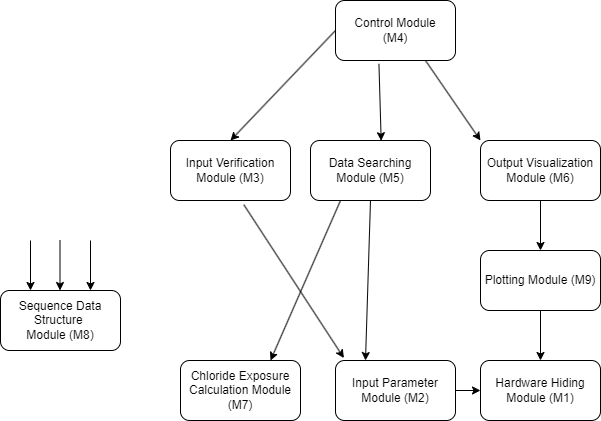
\includegraphics[width=0.7\textwidth]{UsesHierarchy.png}
\caption{Use hierarchy among modules}
\label{FigUH}
\end{figure}

%\section*{References}

\section{User Interfaces}

\begin{figure}[H]
\centering
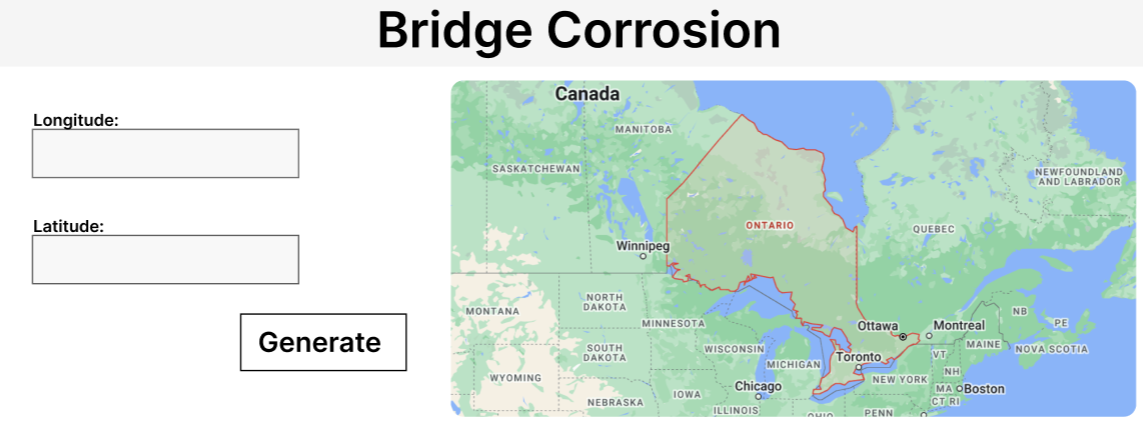
\includegraphics[width=0.9\textwidth]{GUI1.png}
\caption{GUI illustration before inputing coordinate}
\label{FigGUI1}
\end{figure}

\begin{figure}[H]
\centering
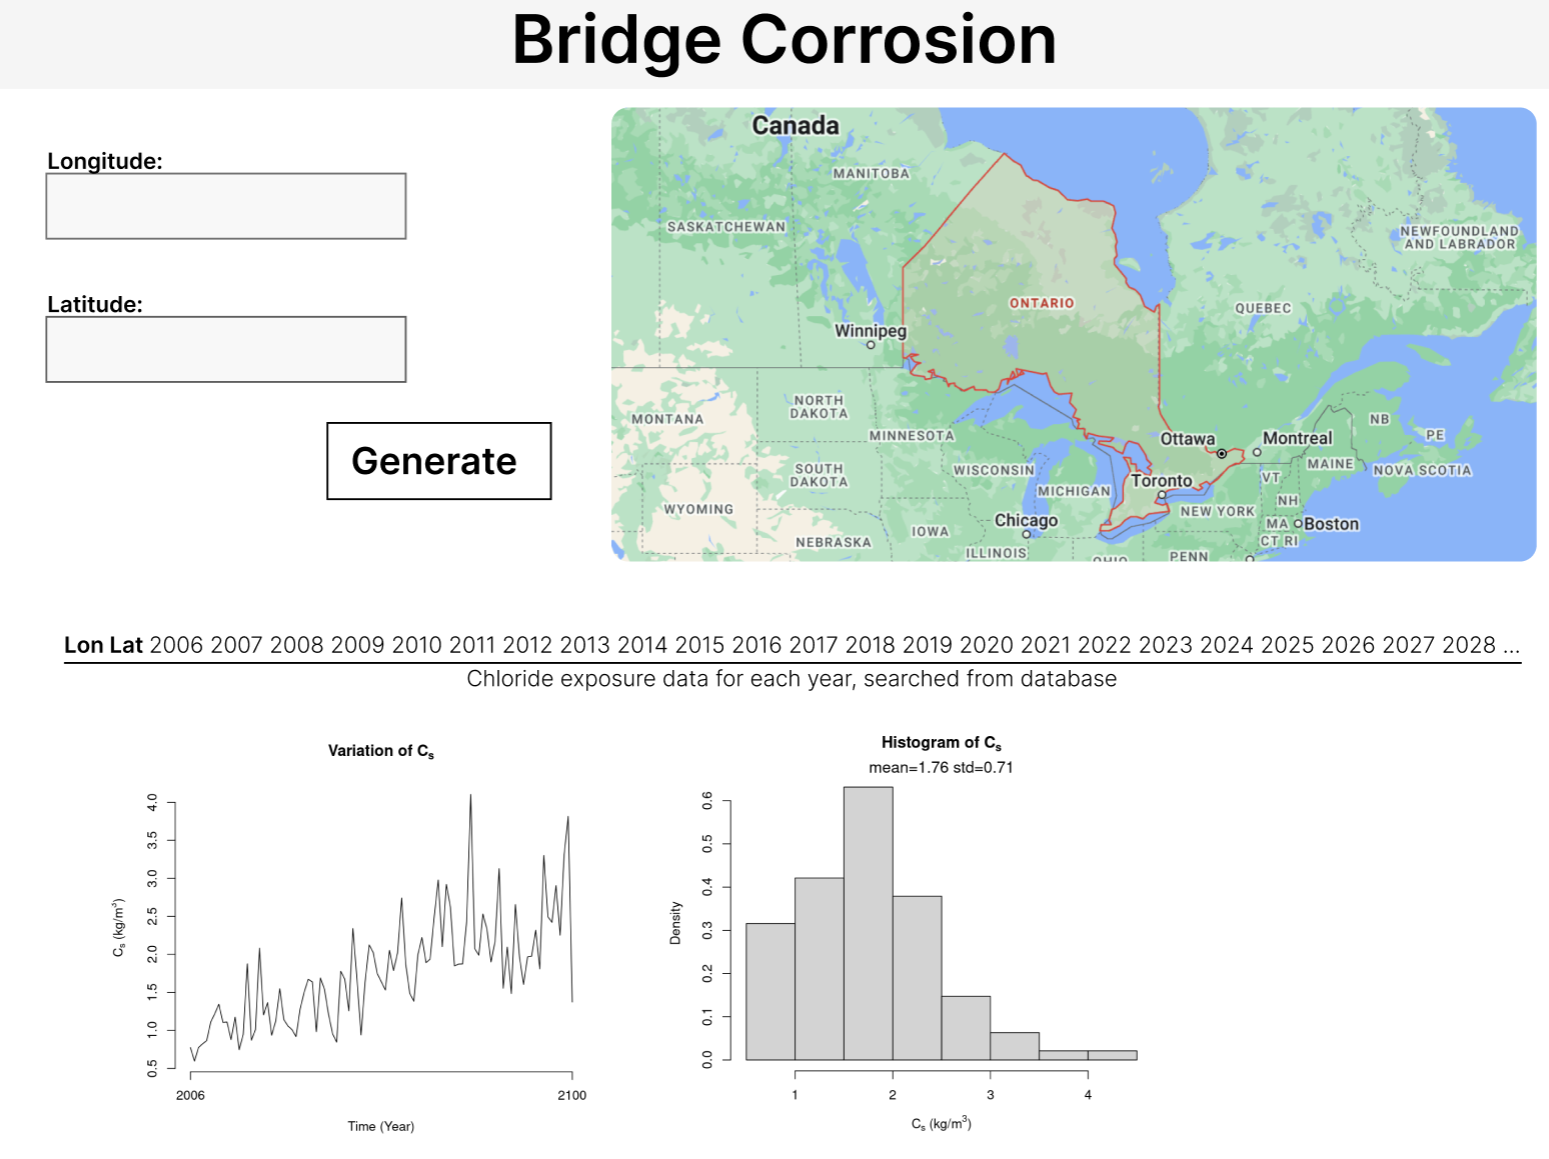
\includegraphics[width=0.9\textwidth]{GUI2.png}
\caption{GUI illustration after inputing coordinate}
\label{FigGUI1}
\end{figure}

\section{Timeline}
The specific timeline is shown in below table:
\begin{table}[H]
\centering
\begin{tabular}{p{0.6\textwidth} p{0.2\textwidth}  p{0.2\textwidth}}
\toprule
 \textbf{Modules} & \textbf{Finish by} & \textbf{Responsible} \\
\midrule
Chloride Exposure Calculation Module & February 25, 2024& Cynthia Liu\\
Input Verification Module & March 5, 2024 & Cynthia Liu\\
Input Parameter Module & March 8, 2024 & Cynthia Liu\\
Data Searching Module & March 20, 2024 & Cynthia Liu\\
Output Visualization Module  & March 27, 2024 & Cynthia Liu\\
Control Module & April 5, 2024 & Cynthia Liu\\

\bottomrule
\end{tabular}
\caption{Timeline}
\end{table}


\section{Appendix}
This section shows the requirements in SRS for quick look up.

\subsection{Functional Requirements}

\begin{itemize}

\item[R\refstepcounter{reqnum}\thereqnum \label{R_Inputs}:] The software should only accept input that is inside Ontario.

\item[R\refstepcounter{reqnum}\thereqnum \label{R_OutputInputs}:] The output need to be a list of data showing the trend of chloride exposure in the past and future at the input location.

\item[R\refstepcounter{reqnum}\thereqnum \label{R_Calculate}:] During the automatic calculation steps, the software should handle situations where units do not match.

\item[R\refstepcounter{reqnum}\thereqnum \label{R_Output}:] The output should be in two decimal points, showing the mass of chloride ions per unit air volume.


\end{itemize}


\subsection{Nonfunctional Requirements}

\noindent \begin{itemize}

\item[NFR\refstepcounter{nfrnum}\thenfrnum \label{NFR_Reliability}:]   \textbf{Reliability}: The predictions generated by the software should be accurate and reliable, reflecting real-world conditions and factors influencing chloride exposure.

\item[NFR\refstepcounter{nfrnum}\thenfrnum \label{NFR_Usability}:] \textbf{Usability}: The software interface should be intuitive and user-friendly, allowing users to easily input coordinates and look at the predicted chloride exposure in the past and future.

\item[NFR\refstepcounter{nfrnum}\thenfrnum \label{NFR_Maintainability}:] \textbf{Maintainability}: The code for this software should be designed and structured in a way that it could be easily comprehended and modified by other potential developers.

\item[NFR\refstepcounter{nfrnum}\thenfrnum \label{NFR_Portability}:]  \textbf{Portability}: This software should be able to run on recent versions of Google Chrome, Firefox, MS Edge and Safari. The operating system include Windows 7+ and Mac OS X 10.7+.

\item[NFR\refstepcounter{nfrnum}\thenfrnum \label{NFR_Scalability}:]   \textbf{Scalability}: The software should be scalable to accommodate potential future expansions or updates, ensuring its continued usefulness as new data or techniques become available.

\end{itemize}


\bibliographystyle {plainnat}
\bibliography{../../../refs/References}

\newpage{}

\end{document}